\documentclass[twoside,leqno,twocolumn]{article}
\usepackage[nocopyright,siamsections,siamtitle,smallbib]{jeffeproc}

% ----------------------------------------------------------------------
%  page dimensions from ltexpprt.sty
% ----------------------------------------------------------------------
%\pretolerance=800
%\tolerance=10000
%\sloppy
%\vsize=55pc
%\hsize=41pc
%\baselineskip=14pt
%\footskip=18pt
\topmargin -24pt
\headheight 12pt
\headsep 17pt
\parskip 1pt plus 1pt minus 1pt
\parindent 1.5em
\textheight 52.5pc  \advance\textheight by \topskip
\textwidth 41pc
\setlength{\oddsidemargin}{-0.875pc}
\setlength{\evensidemargin}{-0.875pc}

%-----------------------------------------------------------------------
%  Necessary packages.
%-----------------------------------------------------------------------
\usepackage{jeffe,graphicx,hyperref}
\usepackage[utf8]{inputenc}
\usepackage{marvosym}
%\usepackage{picins}

%\clubpenalty 5000
%\widowpenalty 5000


%-----------------------------------------------------------------------
%  These packages are purely cosmetic.
%  Just comment them out if they don't work for you.
%-----------------------------------------------------------------------
\usepackage{microtype}
\usepackage[charter]{mathdesign}
\def\sfdefault{fvs}
\def\ttdefault{fvm}
\usepackage[mathcal]{euscript}
\usepackage{stmaryrd}


%-----------------------------------------------------------------------
%  Local definitions
%-----------------------------------------------------------------------
\def\arcto{\mathord\shortrightarrow}
\def\arc#1#2{#1\arcto#2}
\def\cra#1#2{#1\mathord\shortleftarrow#2}
\def\fence#1#2{#1\mathord\shortuparrow#2}
\def\ecnef#1#2{#1\mathord\shortdownarrow#2}
\def\head{\mathit{head}}
\def\tail{\mathit{tail}}
\def\lsh{\mathit{left}}
\def\rsh{\mathit{right}}
\def\rev{\mathit{rev}}
\def\Z{\mathbb{Z}}
\def\Real{\mathbb{R}}
\def\Q{\mathbb{Q}}

% needs marvosym package:
\def\snip{\mathbin{\raisebox{0.15ex}{\rotatebox[origin=c]{60}{\Rightscissors}\!}}}
\def\subsnip{\mathbin{\raisebox{0.15ex}{\rotatebox[origin=c]{60}{\footnotesize\Rightscissors}\!}}}
\def\Gsnip{\mathord{G_{\subsnip}}}

\let\unlhd\trianglelefteq	% fix mathdesign font bug

\let\cycle\gamma
\let\path p
\let\primalarc\alpha
\def\dualarc{p}

\def\Sigmabar{\overline{\smash{\Sigma}\vphantom{t}}}
\def\SIGMABAR{\boldsymbol{\overline{\smash{\Sigma}\vphantom{x}}}}
\def\Gbar{\overline{\smash{G}\vphantom{t}}}
\def\Vbar{\overline{\smash{V}\vphantom{t}}}
\def\Ebar{\overline{\smash{E}\vphantom{t}}}
\def\bbar{\overline{\smash{b}\vphantom{t}}}
\def\nbar{\overline{n}}
\def\gbar{\overline{g}}
\def\wbar{\overline{w}}
\def\sigmabar{\overline{\sigma}}
\def\cyclebar{\overline{\cycle}}
\def\chibar{\overline{\chi}}

\def\paragraph#1{\par\medskip\noindent\textbf{#1}}


\newtheorem{theorem}{Theorem}[section]
\newtheorem{corollary}[theorem]{Corollary}
\newtheorem{lemma}[theorem]{Lemma}

% --------------------------------------------------------------------------------
\pagestyle{empty}
% \markboth{Global Minimum Cuts in Surface Embedded Graphs}
%		 {Jeff Erickson, Kyle Fox, and Amir Nayyeri}

\begin{document}

\title{Global Minimum Cuts in Surface Embedded Graphs}

\author{
	Jeff Erickson%
		\thanks{Portions of this work were done while this author was
				visiting IST Austria.  Research by this author was
				partially supported by NSF grant CCF 09-15519.}
	\hspace{0.5in}
	Kyle Fox%
		\thanks{Portions of this work were done while this author was
				visiting Google, Inc.  Research by this author is
				supported in part by the Department of Energy Office
				of Science Graduate Fellowship Program (DOE SCGF),
				made possible in part by the American Recovery and
				Reinvestment Act of 2009, administered by ORISE-ORAU
				under contract no. DE-AC05-06OR23100.}
	\hspace{0.5in}
	Amir Nayyeri
		\thanks{Portions of this work were done while this author was
				visiting Toyota Technological Institute at Chicago and
				Disney Animation Studio.  Research by this author was partially
				supported by NSF grant CCF 09-15519.}
	\\[1ex]
	\normalsize
	\begin{tabular}{c}
	Department of Computer Science\\
	University of Illinois at Urbana-Champaign\\
	\protect\url{{jeffe,kylefox2,nayyeri2}@cs.uiuc.edu}
	\end{tabular}
}

%\DRAFT

\maketitle

\begin{abstract}
We give a deterministic algorithm to find the minimum cut in a surface-embedded graph in near-linear time. Given an undirected graph embedded on an orientable surface of genus~$g$, our algorithm computes the minimum cut in $g^{O(g)}n \log \log n$ time, matching the running time of the fastest algorithm known for planar graphs, due to Łącki and Sankowski, for any constant~$g$.  Indeed, our algorithm calls Łącki and Sankowski's recent $O(n \log \log n)$ time planar algorithm as a subroutine.

Previously, the best time bounds known for this problem followed from two algorithms for general sparse graphs: a \emph{randomized} algorithm of Karger that runs in~$O(n \log^3 n)$ time and succeeds with high probability, and a deterministic algorithm of Nagamochi and Ibaraki that runs in~$O(n^2 \log n)$ time.  We can also achieve a deterministic $g^{O(g)} n^2 \log \log n$ time bound by repeatedly applying the best known algorithm for minimum $(s,t)$-cuts in surface graphs.  The bulk of our work focuses on the case where the dual of the minimum cut splits the underlying surface into multiple components with positive genus.
\end{abstract}



%---------------------------------------

\section{Introduction}
\label{S:intro}

Recently there has been a new-found interest in flow and cut problems in planar graphs.  While flows in planar graphs have been studied since Ford and Fulkerson's seminal work in the 1950s~\cite{ff-mfn-56}, it has only been a few years since Borradaile and Klein announced the first algorithm to find maximum flows in  directed planar graphs in near-linear time~\cite{b-epnfc-08, bk-amfdp-09}.  Borradaile and Klein’s result came after a long line of work on finding maximum flows and minimum $(s,t)$-cuts in undirected planar graphs~\cite{f-faspp-87, hj-oamfu-85, is-mfpn-79, r-mstcp-83}.  Frederickson’s $O(n\log n)$-time algorithm \cite{f-faspp-87} stood as the fastest algorithm for these problem for almost 25 years, until the recent $O(n\log\log n)$-time algorithm of Italiano \etal~\cite{insw-iamcmf-11}.

There has also been recent work on finding \emph{global} minimum cuts, where
the goal is to partition the vertices of a weighted undirected graph into two non-empty sets, without a specified pair of terminals that must be separated.  (Unless specified otherwise, any references to minimum cuts in this paper refer to this version of the problem.)  Chalermsook, Fakcharoenphol, and Nanongkai described the first deterministic near-linear time algorithm for computing minimum cuts in planar graphs~\cite{cfn-dnlta-04}.  This result was recently improved by Italiano \etal~\cite{insw-iamcmf-11} and again by Łącki and Sankowski~\cite{ls-mcsc-11}, who describe a deterministic algorithm that runs in $O(n \log \log n)$ time.  These algorithms are significantly faster than the best known algorithms for general sparse graphs: a randomized algorithm of Karger that runs in $O(n\log^3 n)$ time and succeeds with high probability~\cite{k-mcnlt-00}, and a deterministic algorithm
of Nagamochi and Ibaraki that runs in $O(n^2 \log n)$ time~\cite{ni-cemcg-92}.

These results and many others support the thesis that planarity aids in finding efficient algorithms.  Moreover, most techniques for efficient computation on planar graphs generalize directly to graphs embedded on surfaces of higher genus, perhaps the most natural generalization of planar graphs.  Examples include minimum spanning trees \cite{p-omst-99, m-tltam-04}; single-source shortest paths \cite{cen-hfcc-09, hkrs-fspap-97, kmw-spdpg-09, lrt-gnd-79, mw-sppgr-10, tm-spltm-09}; multiple-source shortest paths \cite{cc-msspg-07, k-msspp-05}; replacement paths \cite{en-crpsg-11, w-srppp-10}; graph and subgraph isomorphism \cite{g-itegd-00, hw-ltaip-74, m-itgbg-80, e-sipgr-99, e-dtmcg-00}; and approximation of several NP-hard problems~\cite{bdt-ptass-08, bkk-ptass-07, bkk-stpg-07, dhm-aacd-07, e-dtmcg-00}.  However, the first significant progress on flow and cut problems in surface graphs was made only recently~\cite{cen-hfcc-09, cen-mcshc-09, en-mcsnc-11}.  It appears that all our intuitive notions for solving these problems in planar graphs require substantial modification, specifically a significant infusion of topology, when more complicated surfaces are involved.

In this paper, we describe the first deterministic near-linear time algorithm to find global minimum cuts in graphs embedded on orientable surfaces of fixed genus.  Specifically, given an $n$-vertex graph embedded on a surface of genus $g$, our algorithm runs in~$g^{O(g)}n \log \log n$ time.  When the genus $g$ is constant, our algorithm’s running time matches the recent algorithm of Łącki and Sankowski for planar graphs \cite{ls-mcsc-11}.  In fact, our algorithm invokes both Łącki and Sankowski's algorithm and the planar minimum $(s,t)$-cut algorithm of Italiano \etal~\cite{insw-iamcmf-11}.  Further improvements in both of these algorithms would  immediately improve our algorithm as well.

Prior to our work, the fastest algorithms known for computing global minimum cuts in arbitrary surface graphs were the algorithms for general sparse graphs mentioned earlier: Karger’s randomized $O(n \log^3 n)$-time algorithm~\cite{k-mcnlt-00} and Nagamochi and Ibaraki’s $O(n^2 \log n)$-time deterministic algorithm~\cite{ni-cemcg-92}.  For graphs of fixed genus, global minimum cuts can also be computed in 
$g^{O(g)} n^2 \log \log n$ time by invoking the fastest known algorithm for minimum $(s,t)$-cuts in surface graphs $n$ times~\cite{cen-mcshc-09, insw-iamcmf-11}.

At a very high level, the planar-graph algorithms of Chalermsook \etal\ \cite{cfn-dnlta-04} and Łącki and Sankowski use a divide-and-conquer strategy in the dual graph.  In the dual graph, vertices and faces exchange roles; the minimum cut in the primal graph corresponds to the minimum-length cycle in the dual graph.  Their algorithms split the dual graph into two pieces of roughly equal size with a simple cycle, and then recursively compute the minimum length cycle inside each piece.  For the conquering step, Chalermsook \etal\ prove that the minimum-length cycle crosses the boundary between the two pieces at more twice.  They use this fact to argue that a minimum-length cycle crossing the boundary must separate two specific faces and can therefore be found using an algorithm for minimum $(s,t)$-cuts (in the original primal graph).

Unfortunately, this divide-and-conquer approach does not immediately generalize to surfaces with positive genus.  First, the minimum cut is no longer necessarily dual to a single cycle; second, because not all cycles in surface graphs bound disks, we cannot so easily divide the graph into equal-sized pieces that maintain the necessary crossing properties.  To work around these obstacles, as in previous work on $(s,t)$-minimum cuts \cite{cen-mcshc-09, en-mcsnc-11}, we rely on properties of  subgraphs that have minimum weight in their $\Z_2$-homology class.  (Two subgraphs of $G$ are in the same $\Z_2$-homology class if their symmetric difference is the boundary of a subset of faces of $G$; see Section~\ref{S:back} for further details.)  In particular, in Sections~\ref{S:contractible} and~\ref{S:splitting}, we prove several properties of $\Z_2$-minimal subgraphs that can possibly cross the dual of the minimum cut; these properties may be of independent interest.

\subsection{Related work}

\paragraph{\boldmath Minimum $(s,t)$-cuts.}
The first algorithm to compute minimum cuts in planar graphs appears in the seminal work of Ford and Fulkerson~\cite{ff-mfn-56}.  Itai and Shiloach~\cite{is-mfpn-79} proposed an algorithm to compute minimum $(s,t)$-cuts in \emph{undirected} planar graphs in $O(n\log^2 n)$ time.  Their algorithm was later improved by Reif~\cite{r-mstcp-83}, Frederickson~\cite{f-faspp-87}, and most recently Italiano \etal~\cite{insw-iamcmf-11}; the last of these improvements runs in $O(n\log\log n)$ time.  The fastest algorithms known for computing minimum $(s,t)$-cuts in \emph{directed} planar graphs require the computation of maximum $(s,t)$-flows~\cite{b-epnfc-08, bk-amfdp-09}.\footnote{Janiga and Koubek \cite{jk-mcdpn-92} claimed an algorithm to compute minimum $(s,t)$-cuts in directed planar graphs in near-linear time, but their algorithm has a subtle flaw~\cite{kn-mcupg-11}.}  Chalermsook~\etal~\cite{cfn-dnlta-04} described the first algorithm to compute \emph{global} minimum cuts in undirected planar graphs in near-linear time.  Their algorithm was recently improved by Łącki and Sankowski~\cite{ls-mcsc-11} to run in $O(n\log\log n)$ time.

Until recently, the best algorithms to compute minimum cuts in surface graphs were those for general sparse graphs.  Chambers \etal described an algorithm to compute minimum $(s,t)$-cuts in undirected surface graphs in~$g^{O(g)} n \log n$ time~\cite{cen-mcshc-09}.  This time bound was improved to $g^{O(g)} n \log\log n$ Italiano~\etal~\cite{insw-iamcmf-11} and to $2^{O(g)}n\log n$ by Erickson and Nayyeri \cite{en-mcsnc-11}.  For minimum $(s,t)$-cuts in \emph{directed} surface graphs, the fastest algorithm known is the maximum-flow algorithm of Chambers\etal~\cite{cen-hfcc-09}, which runs in near-linear time for graphs of fixed genus and polynomially-bounded integer capacities.

\paragraph{Shortest interesting cycles.}
Itai and Shiloach~\cite{is-mfpn-79} proved that the minimum $(s,t)$-cut in an undirected planar graph $G$ corresponds to the shortest generating cycle in an annulus, obtained by removing the faces~$s^*$ and~$t^*$ from the dual graph $G^*$.  All the planar minimum-cut algorithms mentioned earlier actually work in  this dual formulation.  Thomassen~\cite{t-egnsn-90} described the first polynomial-time algorithm to find the shortest nontrivial cycle in undirected surface graphs; Thomassen’s algorithm runs in $O(n^3)$ time.  Erickson and Har-Peled improved the running time to~$O(n^2 \log n)$ \cite{eh-ocsd-04}.  Their algorithm is currently the best when the genus is unbounded, but there are several faster algorithms when the genus is sufficiently small \cite{cm-fsnsn-07, c-mdpg-10, k-csnco-06, cc-msspg-07, insw-iamcmf-11}.  Cabello~\cite{c-fscss-10} describes an algorithm to find the shortest \emph{simple} contractible cycle (without repeated vertices) in an undirected surface graph in $O(n^2\log n)$ time; he also proves that finding the shortest simple \emph{separating} cycle is NP-hard.  For related results, see \cite{ccl-osaew-10, cdem-fotc-10, ccelw-scsih-08, ew-csec-10}.

Cabello \etal~\cite{ccl-fsncd-10} described the first non-trivial algorithms to compute shortest non-contractible or non-separating cycles in \emph{directed} surface graphs; the fastest of their algorithms runs in~$O(\sqrt{g} n^{3/2}\log n)$ time.  Erickson and Nayyeri~\cite{en-mcsnc-11} showed that a modification of their algorithm for minimum $(s,t)$-cuts finds shortest non-separating cycles in~$2^{O(g)}n\log n$ time.  Most recently, Erickson~\cite{e-sncds-11} proposed algorithms to find shortest non-separating cycles in $O(g^2 n \log n)$ time and to find shortest non-contractible cycles in $g^{O(g)} n \log n$ time.

\paragraph{Shortest equivalent cycles and subgraphs.}
There are several results on finding shortest cycles in surface graphs that are topologically equivalent to a given cycle.  Colin de Verdière and Erickson~\cite{ce-tnpcs-10} described an algorithm to compute the shortest cycle \emph{homotopic} to a given cycle in~$O(gnk \log nk)$ time, where $k$ is the number of edges in the input cycle, generalizing and improving an earlier result of Colin de Verdière and Lazarus for \emph{simple} cycles~\cite{cl-opdsh-07}.

Chambers \etal~\cite{ccelw-scsih-08} showed that finding the shortest cycle (simple or not) in any given \emph{homology} class is NP-hard, but fixed-parameter tractable with respect to genus.  The minimum $(s,t)$-cut algorithms of Chambers \etal~\cite{cen-mcshc-09, en-mcsnc-11} work by computing the minimum-cost \emph{even subgraph} in a given $\Z_2$-homology class, a problem which is also NP-hard.  Chen and Friedman~\cite{cf-qhc-08, cf-hrhl-10} proved that this problem becomes NP-hard to approximate within any constant factor when generalized to simplicial complexes.  Following a strategy first suggested by Sullivan \cite{s-cath-90}, Chambers \etal~\cite{cen-hfcc-09} describe an algorithm to quickly find minimum-cost \emph{circulations} in any given real or integer homology class in a directed surface graph.  Their result was subsequently generalized by Dey \etal~\cite{dhk-ohctu-11} to work with arbitrary chains of arbitrary dimension in arbitrary simplicial complexes.  For more related results, see \cite{cf-mcngh-10, dh-lsako-11, dls-chtl-07, ew-gohhg-05}.

\section{Notation and Terminology}
\label{S:back}

We begin by recalling several useful definitions related to surface-embedded graphs.  For further background, we refer the reader to Gross and Tucker \cite{gt-tgt-01} or Mohar and Thomassen~\cite{mt-gs-01} for topological graph theory, and to Hatcher~\cite{h-at-02} or Stillwell~\cite{s-ctcgt-93} for surface topology and homology.  We adopt most of our terminology and notation from previous works~\cite{cen-mcshc-09, en-mcsnc-11}.

\subsection{Surfaces and Curves}

A \EMPH{surface} (more formally, a \emph{2-manifold with boundary}) is a compact Hausdorff space in which every point has an open neighborhood homeomorphic to either the plane $\Real^2$ or a closed halfplane $\set{(x,y)\in \Real^2\mid x\ge 0}$.  The points with halfplane neighborhoods make up the \EMPH{boundary} of the surface; every component of the boundary is homeomorphic to a circle.

A \EMPH{path} in a surface $\Sigma$ is a continuous function $p\colon [0,1]\to\Sigma$.  An \EMPH{arc} is a path whose endpoints lie on the boundary of $\Sigma$.  A \EMPH{cycle} is a continuous function $\gamma\colon S^1\to\Sigma$.  Paths and cycles are \EMPH{simple} if they are injective.  Following standard practice, we do not distinguish between a simple path or cycle and its image in $\Sigma$.

The \EMPH{genus} of a surface $\Sigma$ is the maximum number of disjoint simple cycles $\gamma_1, \gamma_2, \dots, \gamma_g$ in $\Sigma$ whose complement $\Sigma\setminus(\gamma_1\cup\cdots\cup\gamma_g)$ is connected.  We will consider only compact, connected, orientable surfaces.  Up to homeomorphism, there is exactly one such surface with any genus $g\ge 0$ and any number of boundaries $b\ge 0$; the \EMPH{Euler characteristic $\chi$} of this surface is $\chi := 2-2g-b$.

\subsection{Graph Embeddings}

An \EMPH{embedding} of an undirected graph $G$ on a surface $\Sigma$ maps vertices to distinct points and edges to interior-disjoint curves.  The \emph{faces} of the embedding are maximal connected subsets of $\Sigma$ that are disjoint from the image of the graph.  An embedding is \EMPH{cellular} if each of its faces is homeomorphic to the plane; in particular, in any cellular embedding, each component of the boundary of $\Sigma$ must be covered by a cycle of edges in $G$.  Euler's formula implies that any cellularly embedded graph with $n$ vertices, $m$ edges, and $f$ faces lies on a surface with Euler characteristic $\chi = n-m+f$, which implies that $m = O(n+g)$ and $f=O(n+g)$.  We consider only cellular embeddings of genus $g=O(n)$, so that the overall complexity of the embedding is $O(n)$.

Cellular graph embeddings are equivalent to the \EMPH{combinatorial surfaces} introduced by Colin de Verdi\`ere~\cite{c-rcds-03} and used by several authors to formulate optimization problems for surface-embedded graphs.  A~combinatorial surface consists of an abstract surface $\Sigma$ together with a cellularly embedded graph $G$ with (possibly asymmetrically) weighted edges.  Paths and cycles in a combinatorial surface are directed walks in its graph; the length of any such walk is the sum of its (directed) edge weights, counted with appropriate multiplicity.

Two paths or cycles in a combinatorial surface \EMPH{cross} if no continuous infinitesimal perturbation makes them disjoint; if such a perturbation exists, then the paths are \EMPH{non-crossing}.  We say that a cycle $\gamma$ is \EMPH{non-self-crossing} if no two sub-paths of $\gamma$ cross, \EMPH{weakly simple} if $\gamma$ is non-self-crossing and traverses each edge at most once, and \EMPH{(strictly) simple} if $\gamma$ visits each vertex at most once.

We redundantly use the term \EMPH{arc} to refer to a walk in the graph whose endpoints are boundary vertices.  Likewise, we use the term \EMPH{cycle} to refer to a closed walk in the graph.  \EMPH{Cutting} a combinatorial surface along a cycle or  arc modifies both the surface and the embedded graph.  For any combinatorial surface $S = (\Sigma, G)$ and any cycle or arc $\gamma$ in~$G$, we define a new combinatorial surface \EMPH{$S \snip \gamma$} by taking the topological closure of $\Sigma \backslash \gamma$ as the new underlying surface; the new embedded graph contains two copies of each vertex and edge of $\gamma$, each bordering a new boundary.  In contrast, a \EMPH{cut} in a \emph{graph} is a set of edges whose removal partitions the graph into two non-empty connected components.  The weight of a cut is the total weight of its edges.

\subsection{Homotopy and Homology}

Two cycles $\gamma$ and $\delta$ in $\Sigma$ are \emph{homotopic}, or in the same \emph{homotopy class}, if there is a continuous map $h\colon {[0,1]\times S^1 \to \Sigma}$ such that $h(0,\cdot) = \gamma$ and $h(1,\cdot) = \delta$.  The function $h$ is called a \emph{homotopy} between $\gamma$ and~$\delta$.  A cycle $\gamma$ is \EMPH{contractible} if it is homotopic to a constant map, \EMPH{separating} if $\Sigma\setminus\gamma$ is disconnected, and \EMPH{splitting} if $\Sigma\setminus\gamma$ is disconnected and both components have positive genus.
Similarly, two arcs $\alpha$ and $\beta$ are homotopic if there is a continuous  map $h\colon {[0,1]\times[0,1] \to \Sigma}$ such that ${h(0,\cdot) = \alpha}$, $h(1,\cdot) = \beta$, and $h(t,\cdot)$ is an arc for all $t\in [0,1]$.  

An arc or a cycle is \EMPH{tight} if it is as short as possible in its homotopy class.  A \EMPH{system of tight arcs} is a minimal set $\set{\alpha_1, \alpha_2, \dots, \alpha_k}$ of arcs such that $\Sigma \snip P$ is a disk and each arc $\alpha_i$ is tight.  Euler’s formula implies that any system of tight arcs contains exactly $2g+b-1$ arcs.

%\color{green} The set of homotopy classes of loops in $\Sigma$ with basepoint $x$ defines a group $\pi_1(\Sigma,x)$ under concatenation, called the \emph{fundamental group} of $\Sigma$ at point $x$.
%\color{black}

Homology is a coarser equivalence relation than homotopy, with nicer algebraic properties. Like several earlier papers \cite{cf-qhc2-07, cf-qhc-08, dls-chtl-07, dlsc-cgaht-08, cen-mcshc-09, en-mcsnc-11}, we consider only one-dimensional cellular homology with coefficients in the finite field $\Z_2$; this restriction allows us to radically simplify our definitions.

Fix a cellular embedding of an undirected graph $G$ on a surface $\Sigma$ with genus $g$.  An \EMPH{even subgraph} is a subgraph of $G$ in which every node has even degree, or equivalently, the union of edge-disjoint cycles.  An even subgraph is \EMPH{null-homologous} if it is the boundary of the union of a subset of faces of $G$.  In this paper, the term \EMPH{separating subgraph} always refers to a null-homologous even subgraph with at least one edge.  Two even subgraphs $\eta$ and $\eta'$ are \EMPH{homologous}, or in the same \EMPH{homology class}, if their symmetric difference \EMPH{$\eta\oplus\eta'$} is null-homologous.  The even subgraphs of $G$ fall into exactly $4^g$ $\Z_2$-homology classes.

We define the \EMPH{carrier} of a (not necessarily simple) cycle $\cycle$ in~$G$ to be the even subgraph of edges that~$\cycle$ traverses an odd number of times; two cycles are homologous if their carriers are homologous.  A cycle~$\cycle$ or even subgraph~$\eta$ is \EMPH{$\Z_2$-minimal} if it has minimum total length among all cycles or even subgraphs homologous with $\cycle$ or $\eta$.

%The homotopy and homology class of an arc or a cycle is the homotopy and homology of its corresponding paths on the surface, respectively.  

\subsection{Graph Duality}

For any graph $G$ on a surface without boundary, we can define a canonical \EMPH{dual graph $G^*$}.  The vertices of $G^*$ correspond to the faces of $G$, and two vertices in $G^*$ are joined by a (dual) edge if and only if the corresponding faces of~$G$ are separated by an edge of $G$.  Thus, every edge~$e$ in~$G$ has a corresponding dual edge in $G^*$, denoted~\EMPH{$e^*$}.  For any face $f$ of~$G$, we let $f^*$ denote the corresponding vertex of $G^*$.  The dual graph $G^*$ has a cellular embedding on $\Sigma$, whose faces correspond exactly to the vertices of $G$.  For any vertex $v$ of~$G$, we let $v^*$ denote the corresponding face of $G^*$.  Duality is an involution---the dual of $G^*$ is isomorphic to the original graph~$G$.

\begin{figure}[htb]
\centering
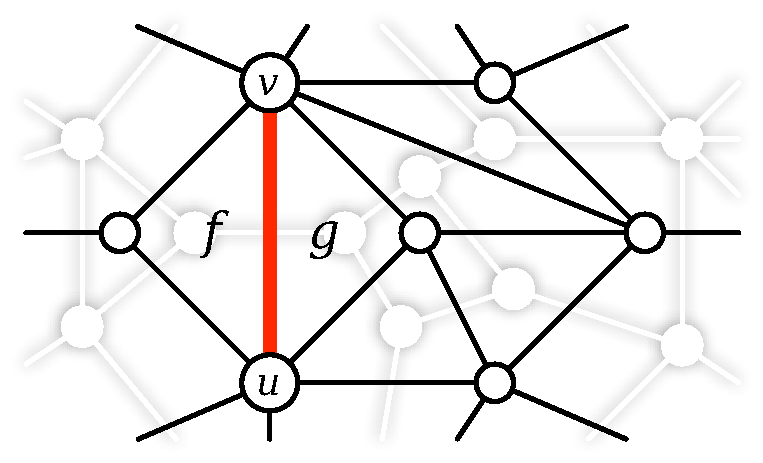
\includegraphics[height=0.9in]{Fig/primal}\quad
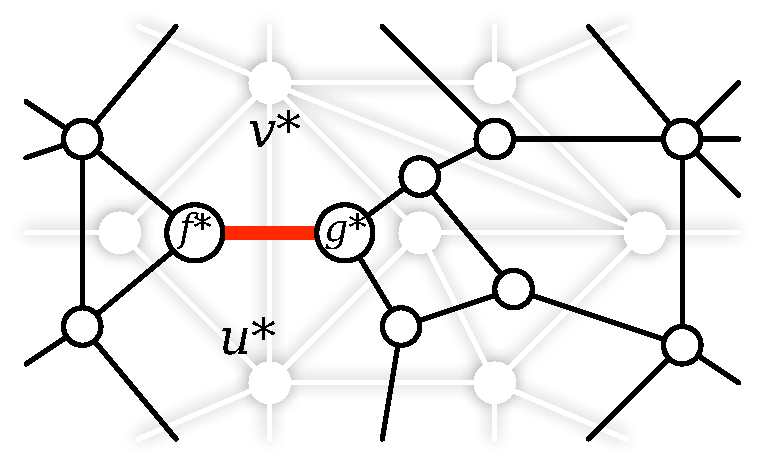
\includegraphics[height=0.9in]{Fig/dual}
\caption{Graph duality.  One edge $uv$ and its dual $(uv)^* =
f^*g^*$ are emphasized.} \label{F:primaldual}
\end{figure}

%
%When the graph $G$ is fixed, we abuse notation by writing $H^*$ to denote the subgraph of $G^*$ containing the edges dual to the edges of a subgraph $H$ of $G$.  If a subgraph $C^*$ is separating, then its dual $C$ is a \EMPH{cut}.
%

%\color{green}
%Any undirected graph $G$ embedded on a surface $\Sigma$ with boundary has a \EMPH{dual graph~$G^*$}, defined as follows.\footnote{Our definition differs slightly from the one proposed by Erickson and Colin de Verdi\`ere~\cite{octagons}.}  The dual graph~$G^*$ has a vertex $f^*$ for each face $f$ of~$G$, \emph{including the boundary cycles}, and an edge $e^*$ for each edge in $G$, including the boundary edges.  For each boundary cycle $\delta$ of~$G$, we refer to the corresponding vertex $\delta^*$ of $G^*$ as a \EMPH{dual boundary vertex}.  The dual graph $G^*$ has a natural cellular embedding in the surface~\EMPH{$\Sigma^\bullet$} obtained from $\Sigma$ by gluing a disk to each boundary cycle; each face of this embedding corresponds to a vertex of $G$.  See Figure \ref{F:duality}.  (Duality can be extended to directed graphs~\cite{surflow}, but our results do not require this extension.)
%\color{black}
%\begin{figure}[htb]
%\centering
%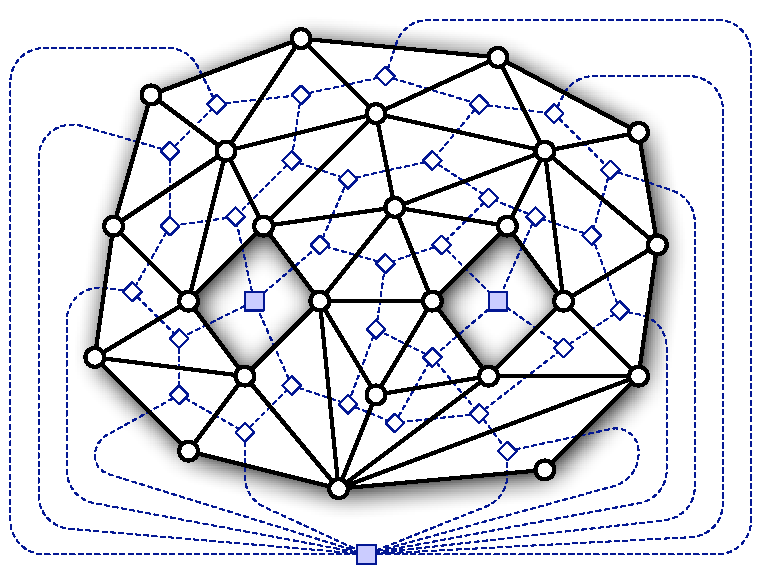
\includegraphics[scale=0.45]{Fig/pants}
%\caption{A cellularly embedded graph $G$ (solid lines) on a pair of pants (genus 0 with 3 boundaries), and its dual graph $G^*$ (dashed lines).  Dual boundary vertices are indicated by squares.}
%\label{F:duality}
%\end{figure}

For any subgraph $F = (U,D)$ of $G = (V,E)$, we write \EMPH{$G\setminus F$} to denote the edge-complement of~$F$ in~$G$ or~${(V, E\setminus D)}$.  Also, when the graph $G$ is fixed, we abuse notation by writing~$F^*$ to denote the subgraph of $G^*$ corresponding to a subgraph $F$ of~$G$; each edge in $F^*$ is the dual of a unique edge in~$F$.  In particular, we have the identity $(G\setminus F)^* = G^* \setminus F^*$.

%\color{green}
%For most of the problems we consider, the input consists of a \emph{directed} edge-weighted graph $G$ with a cellular embedding on some surface.  We use the notation \EMPH{$\arc{u}{v}$} to denote the directed edge from vertex $u$ to vertex $v$.  Without loss of generality, we consider only \emph{symmetric} directed graphs, in which the reversal $\arc{v}{u}$ of any edge $\arc{u}{v}$ is another edge.  We also assume that in the cellular embedding, the images of any edge and its reversal coincide (but with different orientations).  Thus, like Cabello \etal \cite[Section 2.3]{ccl-fsncd-10}, we implicitly model directed graphs as \emph{undirected graphs with asymmetric edge weights}.
%\color{black}



%--------------------------------------

\section{Homology Cuts}
\label{s:homology}

We are now ready to describe our minimum cut algorithm.  To work with the topology of~$\Sigma$ in computing a minimum cut, we use the following modification of a lemma of Chambers~\etal~\cite[Lemma~3.1]{cen-mcshc-09}.  Recall that a \emph{separating subgraph} is a null-homologous even subgraph with at least one edge.

\begin{lemma}
\label{L:mincut-z2}
Let~$G$ be an undirected graph with non-negative edge capacities, cellularly   embedded on a surface~$\Sigma$ without boundary, and let~$C$ be a minimum-capacity   cut in~$G$.  Then~$C^*$ is a minimum-weight separating subgraph of~$G^*$.
\end{lemma}

\begin{proof}
  Let~$C$ be an arbitrary cut in~$G$.  The cut partitions the vertices of $G$
  into two disjoint subsets~$S$ and~$T$. Therefore, the dual subgraph~$C^*$
  partitions the faces of~$G^*$ into two disjoint subsets~$S^*$ and~$T^*$.
  Further,~$C^*$ is the boundary of the union of faces in~$S^*$, implying
  that~$C^*$ is null-homologous in~$\Sigma$ and therefore separating.

  Conversely, let~$C^*$ be an arbitrary separating subgraph of~$G^*$.
  As~$C^*$ is null-homologous, it is the boundary of a subset of the faces
  of~$G^*$.  Moreover, because $C^*$ is non-empty, it must be the boundary of
  a \emph{proper, non-empty} subset of faces.  Let $s^*$ and $t^*$ be faces
  of $G^*$ on either side of $C^*$.  Any path from~$s$ to~$t$ in the primal
  graph~$G$ must traverse at least one edge of~$C$.  We conclude that~$C$ is
  a cut (in particular, an $(s,t)$-cut).
\end{proof}

Fix an undirected graph~$G=(V,E)$, a non-negative weight function~$w\colon E\to \Real$, and a cellular embedding of~$G$ on a surface~$\Sigma$ of genus~$g$ with at least two faces.  In light of Lemma \ref{L:mincut-z2}, we focus our attention on finding a minimum-weight separating subgraph of~$G$. 

To simplify our exposition, we assume without loss of generality that $G$ contains a unique shortest path between any pair of vertices; this assumption can be enforced with high probability using standard perturbation techniques~\cite{mvv-memi-87}.

 Our algorithm separately considers three (overlapping) cases, illustrated in Figure~\ref{F:3cases}:
\begin{enumerate}
  \item
    Some minimum-weight separating subgraph is the union of two nonempty edge-disjoint even subgraphs.
  \item
    Some minimum-weight separating subgraph consists of a single contractible simple cycle.
  \item
    Every minimum-weight separating subgraph splits the surface into two components of positive genus.
\end{enumerate}
%
\begin{figure}[hb]
\centering
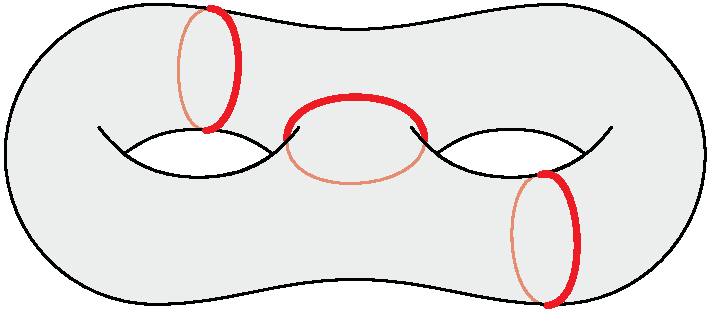
\includegraphics[height=1in]{Fig/homologous1}\\[1ex]
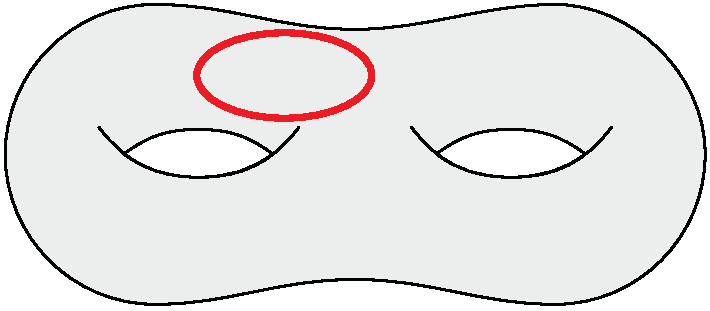
\includegraphics[height=1in]{Fig/shortcon2}\\[1ex]
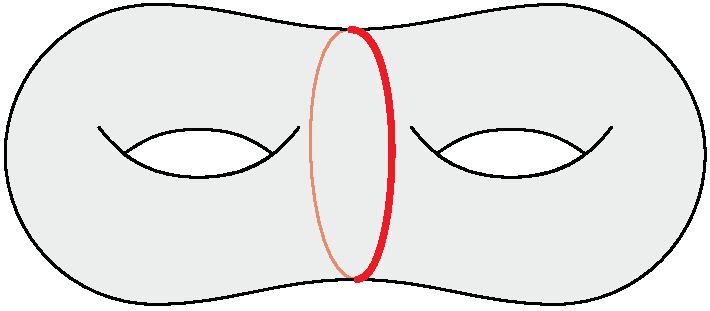
\includegraphics[height=1in]{Fig/shortsep2}\\[1ex]
\caption{Three types of minimum-weight separating subgraphs: decomposable, contractible, and splitting.}
\label{F:3cases}
\end{figure}
%

We emphasize that only the first two cases are disjoint.  In the following sections, we describe subroutines to find a minimum-weight separating subgraph if the corresponding condition holds.  If one of these conditions does not hold, the corresponding subroutine returns either an error or a separating subgraph that is not minimal.  By running all three subroutines and returning the best result, we find a minimum separating subgraph no matter which category it falls into.

\section{Multiple Even Subgraphs}

We begin with the easiest of the three cases.  If the minimum separating subgraph
$\sigma$ is the union of multiple non-empty even subgraphs, the following algorithm finds it.  Otherwise, this algorithm may return an even subgraph more expensive
than~$\sigma$.

\begin{lemma}
\label{L:minimum-cycle}
Let $\sigma$ be a minimum-weight separating subgraph of $G$.  If $\sigma$ is the union of two or more non-empty even subgraphs, then $\sigma$ is also the union of a non-separating $\Z_2$-minimal subgraph $\eta$ and a minimum-weight even subgraph that is edge-disjoint from $\eta$ and homologous with $\eta$.
\end{lemma}

%\begin{lemma}
%\label{L:minimum-cycle}
%  Let~$\sigma$ be a minimum separating subgraph of~$G$. If~$\sigma$
%  can be decomposed into the carriers of two or more cycles, then
%  there exists a decomposition of~$\sigma$ that is composed of the carrier for a
%  non-separating
%  $\Z_2$-minimal cycle~$\alpha$ of homology
%  class $h$ and a minimum-weight even subgraph that is disjoint
%  from~$\alpha$ and in the homology class $h$.
%\end{lemma}

%\begin{lemma}
%\label{L:minimum-cycle}
%  Let~$X$ be a minimum separating subgraph of~$G$. If~$X$
%  decomposes into the carriers of two or more cycles, then
%  there exists a decomposition of~$X$ that is composed of the carrier for a
%  non-separating
%  $\Z_2$-minimal cycle~$C$ and a minimum-weight even subgraph that is disjoint
%  from~$C$ and in the same homology class as~$C$.
%\end{lemma}


\begin{proof}
Suppose $\sigma$ is the union of two non-empty edge-disjoint even subgraphs $\gamma$ and $\delta$.  Because $\sigma$ is null-homologous, $\gamma$ and $\delta$ must be homologous.  Let $\eta$ be the minimum-weight even subgraph homologous to $\delta$ and~$\gamma$.  If either $\eta = \delta$ or $\eta = \gamma$, we are done.  Otherwise, $\eta\oplus\gamma$ is a separating subgraph of smaller total weight than $\sigma$, which is impossible.
\end{proof}

The minimum even subgraph in any homology class can be found in $g^{O(g)} n \log \log n$ time using Italiano \etal's modification
of an algorithm by Chambers, Erickson, and Nayyeri~\cite{cen-mcshc-09, insw-iamcmf-11}.
Likewise, we can find the smallest subgraph of any homology class that avoids
the minimum even subgraph $\eta$ in that same class in $g^{O(g)} n \log \log n$ time
by assigning infinite weight to every edge of $\eta$ and applying the same algorithm.
We can enumerate $\Z_2$-homology classes and apply
Lemma~\ref{L:minimum-cycle} to show the following:
%
%Erickson and Nayyeri give~$2^{O(g)}n\log n$ time algorithms to compute shortest
%cycles in any homology class as well as smallest even subgraphs in any
%homology class. By running both of these algorithms~$2^{2g}$ times, we
%immediately get the following lemma.

\begin{lemma}
\label{L:solution-multi}
  We can compute a minimum-weight separating subgraph in $g^{O(g)} n \log \log n$
  time, if any such subgraph is the union of two non-empty edge-disjoint
  even subgraphs.
\end{lemma}

%In the next section, we consider the case where every minimum
%separating subgraph is the carrier of a single cycle.

\section{Contractible Cycle}
\label{S:contractible}

Next we describe an algorithm to handle the case where some minimum-weight separating subgraph is a contractible simple cycle.  We emphasize that out algorithm may fail to return a contractible simple cycle if no such cycle is a minimum separating subgraph.  We begin by borrowing a result of Cabello~\cite[Lemma 4.1]{c-fscss-10}.

\begin{lemma}[Cabello~\cite{c-fscss-10}]
\label{L:disjoint-tight-arc}
Let $\alpha$ be a tight arc or tight cycle on $G$.  The shortest contractible simple cycle does not cross $\alpha$.
\end{lemma}

\begin{corollary}
\label{C:disjoint-sep-cycle}
The shortest contractible simple cycle and the shortest non-separating cycle in $G$ do not cross.
\end{corollary}

\begin{figure}[h]
\centering
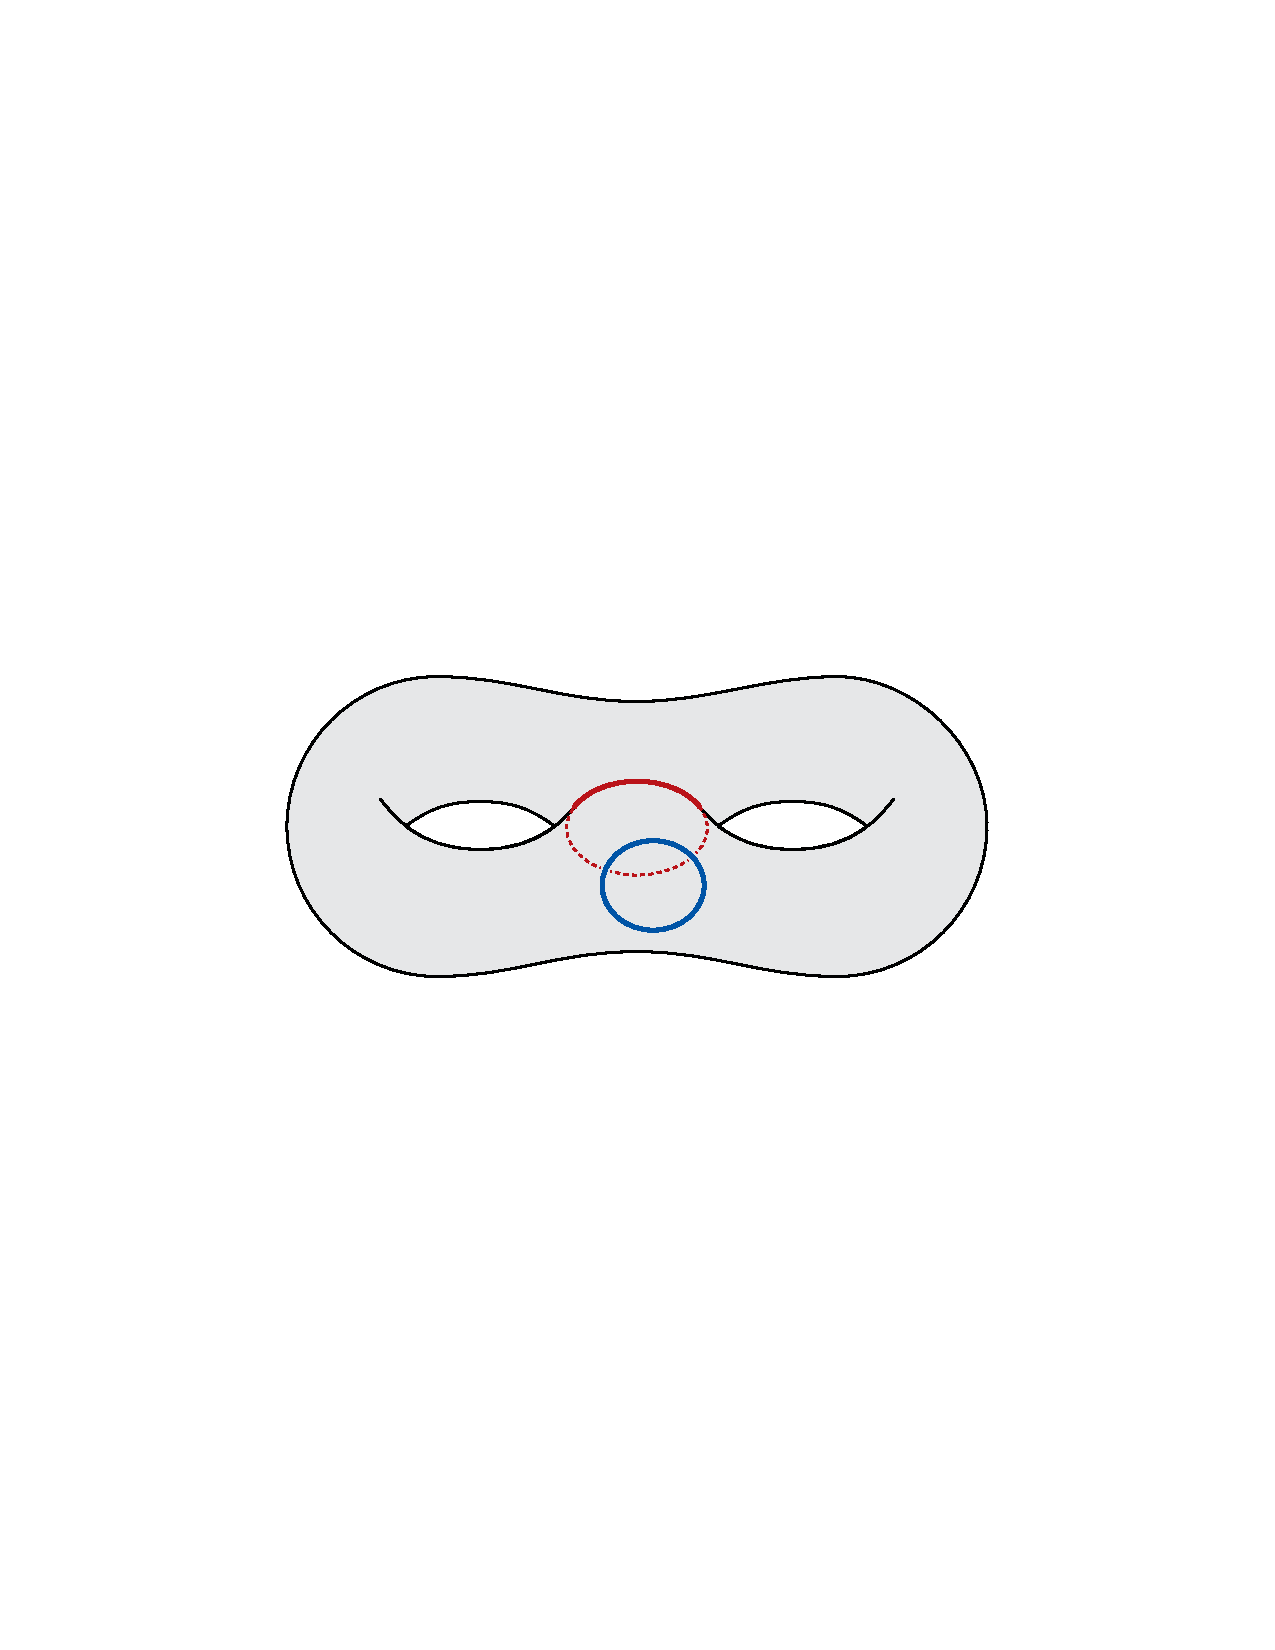
\includegraphics[height=1.2in]{Fig/shortcon-vs-shortnonsep}
\caption{The shortest contractible simple cycle does not cross the shortest non-separating cycle.}
\label{F:forbidden-pair}
\end{figure}

%\begin{proof}
%Erickson and Nayyeri~\cite{cen-surfcut-09} describe an algorithm to compute the minimum member of a given $\Integer_2$-homology class in $g^{O(g)} n \log n$ time.  They reduce the problem to computing $g^{O(g)}$ shortest paths in a covering space and call Kutz~\cite{k-csnco-06} algorithm to find those shortest paths.  Kutz's algorithm, in turn, calls Frederickson's algorithm that computes planar minimum cut in $O(n \log n)$ time~\cite{f-faspp-87}.
%
%Recently, Italialno et. al.~\cite{insw-iamcmf-11} describe an $O(n \log\log n)$ time algorithm to compute planar minimum cut.  It follows that the minimum member of a given homology class can be computed in $g^{O(g)} n \log\log n$ time.  The shortest non-separating cycle is the shortest cycle that is neither null-homologous nor homologous to a boundary.  Therefore, it can be found in the same asymptotic running time through brute force.
%\end{proof}

\begin{lemma}
\label{L:contractible-alg}
  We can compute a minimum-weight separating subgraph in $g^{O(g)} n \log \log n$
  time, if any such subgraph is a contractible simple cycle.
\end{lemma}

\begin{proof}
We begin by computing the shortest non-separating cycle~$\alpha$ in $G$ in $g^{O(g)}n \log \log n$ time, using a recent modification of an algorithm of Kutz~\cite{k-csnco-06} by Italiano \etal~\cite{insw-iamcmf-11}.  The surface $\Sigma \snip \alpha$ has two boundary cycles $\alpha'$ and $\alpha''$.  We compute a system $P$ of tight arcs connecting $\alpha'$ and $\alpha''$ in $O(n)$ time using the shortest-path algorithm of Henzinger \etal~\cite{hkrs-fspap-97}, as described by Erickson and Nayyeri \cite{en-mcsnc-11}.  Let $\Gsnip$ denote the planar graph $G \snip (\alpha \cup P)$; this graph has $O(gn)$ vertices.

Pick an arbitrary edge $e$ of $\alpha$, and let $e_1$ and $e_2$ be the copies of $e$ in~$\Gsnip$.  Let $\gamma_1$ and $\gamma_2$ be the shortest simple cycles in the  subgraphs $\Gsnip \backslash e_1$ and $\Gsnip \backslash e_2$, respectively.  We  compute both~$\gamma_1$ and~$\gamma_2$ in $O(gn \log\log n)$ time using the algorithm of Łącki and Sankowski~\cite{ls-mcsc-11}.

Let~$\gamma$ the shorter of the cycles~$\gamma_1$ and $\gamma_2$.  The cycle~$\gamma$ projects to a null-homologous closed walk $\gamma'$ in the original graph $G$, which may or may not be simple.  The outer face of $\Gsnip$ is the only face that is not also a face of~$G$.  It follows that the only separating cycle in $\Gsnip$ that is not a separating subgraph in $G$ is the boundary of outer face.  Because $\gamma$ avoids at least one edge of the outer face, the carrier of $\gamma'$ must be non-empty.

Corollary~\ref{C:disjoint-sep-cycle} and Lemma~\ref{L:disjoint-tight-arc} imply that some shortest contractible simple cycle $\sigma$ in $G$ crosses neither~$P$ nor $\alpha$.  (We emphasize that our algorithm does not actually compute~$\sigma$.)  This cycle $\sigma$ appears as a simple cycle in $\Gsnip$ that avoids at least one of the edges $e_1$ or $e_2$.  Thus, $\sigma$ cannot be shorter than $\gamma$.  

\begin{figure}[ht]
\centering
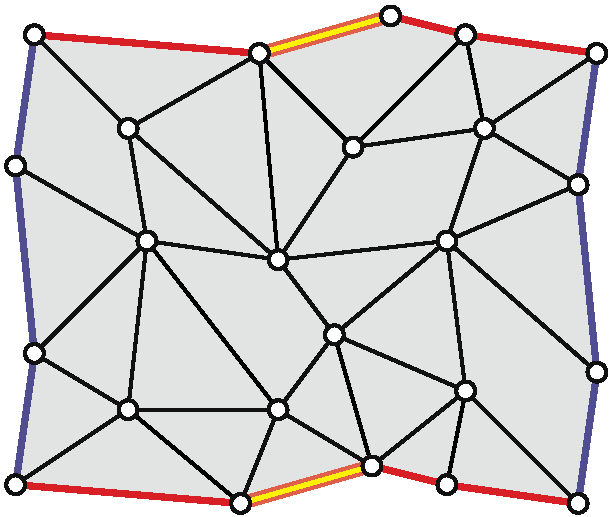
\includegraphics[height=1.2in]{Fig/forbidden-pair}
\caption{At least one copy of $e$ is forbidden in the planarized graph.}
\label{F:forbidden-pair}
\end{figure}

If the walk $\gamma'$ is a simple cycle, it must be contractible, and therefore cannot be shorter than $\sigma$.  In this case, $\gamma'$ must be a shortest contractible simple cycle in $G$, and our algorithm returns this cycle.  On the other hand, if $\gamma'$ is not a simple cycle, its carrier is composed of more than one cycle; in this case, our algorithm reports correctly that no minimum-weight separating subgraph of $G$ is a contractible simple cycle.
\end{proof}


\section{Splitting Subgraph}

\label{S:splitting}
Finally, we consider the case where every minimum-weight separating subgraph splits the surface into two components with genus.  Our algorithm may not return the minimum-weight splitting subgraph if it is not the minimum-weight separating subgraph, but it always returns some separating subgraph if it returns anything at all.

\begin{lemma}
  \label{L:split-nocross}
  Suppose every minimum-weight separating subgraph is splitting;
  let $\sigma$ be a minimum-weight separating subgraph.
  Let~$\gamma$ be a closed walk on~$G$ such that~$\sigma$
  does not cross~$\gamma$, and let~$\eta$ be the
  shortest even subgraph homologous to~$\gamma$.
  Then~$\eta$ lies in the closure of the same component
  of~$\Sigma \setminus \sigma$ as~$\gamma$.
\end{lemma}

\begin{proof}
Assume for the sake of deriving a contradiction that~$\eta$ does not lie in the closure of the same component as~$\gamma$.  The subgraph~$\sigma$ separates the faces of~$G$ into two non-empty sets.  Call the faces in the component of~$\Sigma \setminus \sigma$ containing~$\gamma$ the \emph{near} faces and call the rest of the faces  \emph{far}.  Similarly, the even subgraph $\eta \oplus \gamma$ is null-homologous and separates the faces of $G$ into two subsets; call the faces in one subset \emph{black} and the others \emph{white}.

\begin{figure}[h]
\centering
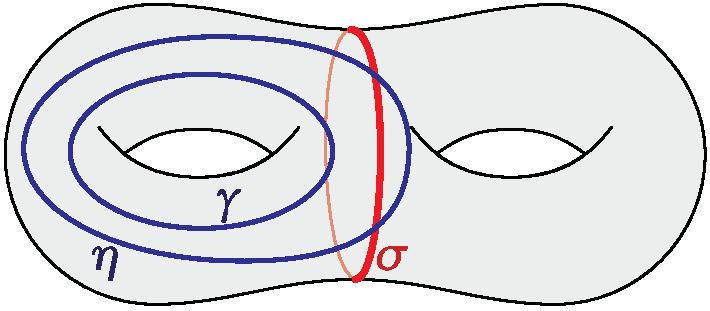
\includegraphics[height=1.2in]{Fig/lemma61}
\caption{An impossible crossing: the shortest separating cycle $\sigma$, a cycle~$\gamma$ that avoids $\sigma$, and the shortest even subgraph $\eta$ homologous to $\gamma$.}
\label{F:lemma61}
\end{figure}

Let~$F$ be the boundary of the union of the far black faces in $G$.  By definition,~$F$ is a null-homologous even subgraph.  By assumption, $\eta$ has edges that are incident to two far faces, but $\gamma$ does not; thus, there is at least one far black face.  Since there is also at least one white face, $F$ is non-empty.  Because both~$F$ and $\sigma$ are null-homologous, the even subgraph $\eta' = \eta \oplus F \oplus \sigma$ is homologous to $\eta$, and therefore to $\gamma$.

For any subgraph~$H$ of $G$, let $w(H)$ denote the sum of the weights of the edges of $H$.  We now prove that $w(F) + w(\eta') \leq w(\eta) + w(\sigma)$ by bounding the contribution of each edge $e \in E(G)$ to both sides of the inequality.  Note that both $F$ and $\eta’$ are subgraphs of $\sigma\cap \eta$; moreover, $F \oplus \eta’ = \sigma \oplus \eta$.  There are three cases to consider.
\begin{itemize}
\item
If $e \not\in \eta \cup \sigma$, then $e \not\in F$.  In this case, $e$ contributes $0$ to both sides of the inequality.
\item
If $e \in \sigma \oplus \eta$, then $e \in F \oplus \eta’$.  In this case, $e$ contributes $w(e)$ to both sides of the inequality.
\item
If $e \in \sigma \cap \eta$, then $e$ contributes exactly $2w(e)$ to the right side of the inequality.  Trivially, $e$ contributes at most $2w(e)$ to the left side.
\end{itemize}

On the other hand, because $F$ is a separating subgraph, we must have $w(F) > w(\sigma)$.  It immediately follows that $w(\eta') < w(\eta)$, which contradicts the minimality of $\eta$.
\end{proof}

\begin{corollary}
\label{C:split}
Suppose every minimum-weight separating subgraph is splitting; let $\sigma$ be a minimum-weight separating subgraph.  Then $G$ contains two even subgraphs $\eta_1$ and~$\eta_2$ that lie in the closures of different components of $\Sigma \setminus \sigma$, such that $\eta_1$ and $\eta_2$ are minimal in their respective nontrivial homology classes.
\end{corollary}

%  \label{C:split-cycles}
%  Suppose the minimum separating subgraph~$\sigma$ is splitting.
%  There exist two
%  non-crossing
%  closed walks~$\alpha_1$ and~$\alpha_2$ such that~$\alpha_1$
%  and~$\alpha_2$ can be embedded in the closures of different components
%  of~$\Sigma \setminus \sigma$
%  and~$\alpha_1$ and~$\alpha_2$ are minimal in their respective nontrivial
%  homology classes.

\begin{proof}
  Let $\Sigma_1$ and $\Sigma_2$ denote the closures of the components of
  $\Sigma \setminus \sigma$.  Let $\gamma_1$ be any closed walk in $\Sigma_1$
  whose homology class is nontrivial; such a closed walk exists because
  $\Sigma_1$ has positive genus.  Lemma~\ref{L:split-nocross} implies that
  the shortest even subgraph~$\eta_1$ in $G$ that is homologous to~$\gamma_1$
  lies in $\Sigma_1$.  Similarly, $\Sigma_2$ contains the shortest even
  subgraph of~$G$ that is homologous to any nontrivial closed walk in $\Sigma_2$.
\end{proof}

\begin{lemma}
  \label{L:split-alg}
  We can compute a minimum-weight separating subgraph in $g^{O(g)} n \log \log n$
  time, if every such subgraph is splitting.
\end{lemma}

Before we prove the lemma, we describe the following subroutine.
Given two non-crossing closed walks~$\alpha_1$ and~$\alpha_2$ in
distinct $\Z_2$-homology classes, we show how to compute
in $g^{O(g)}n \log \log n$ time the minimum non-empty even
subgraph~$\sigma$ that separates~$\alpha_1$ and~$\alpha_2$ if it exists.

We compute the graph $\Gsnip = G \snip (\alpha_1\cup \alpha_2)$ in linear
time. Let~$\Sigma_{\subsnip}$ be its underlying surface.
The graph~$\Gsnip$ has genus~$g-2$ and
four boundary cycles~$\alpha'_1$, $\alpha''_1$, $\alpha'_2$,
and~$\alpha''_2$. An even subgraph separating~$\alpha_1$ and~$\alpha_2$
in~$G$ corresponds to an even subgraph in~$\Gsnip$ that is homologous
to $\alpha'_1 \oplus \alpha''_1$. Unfortunately, we cannot simply find the
smallest even subgraph of~$\Gsnip$ homologous to
$\alpha'_1 \oplus \alpha''_1$
as this subgraph might correspond to an empty subgraph of~$G$.  Instead, we employ
a technique similar to the one used in Lemma~\ref{L:contractible-alg}.

\begin{figure}[ht]
\centering
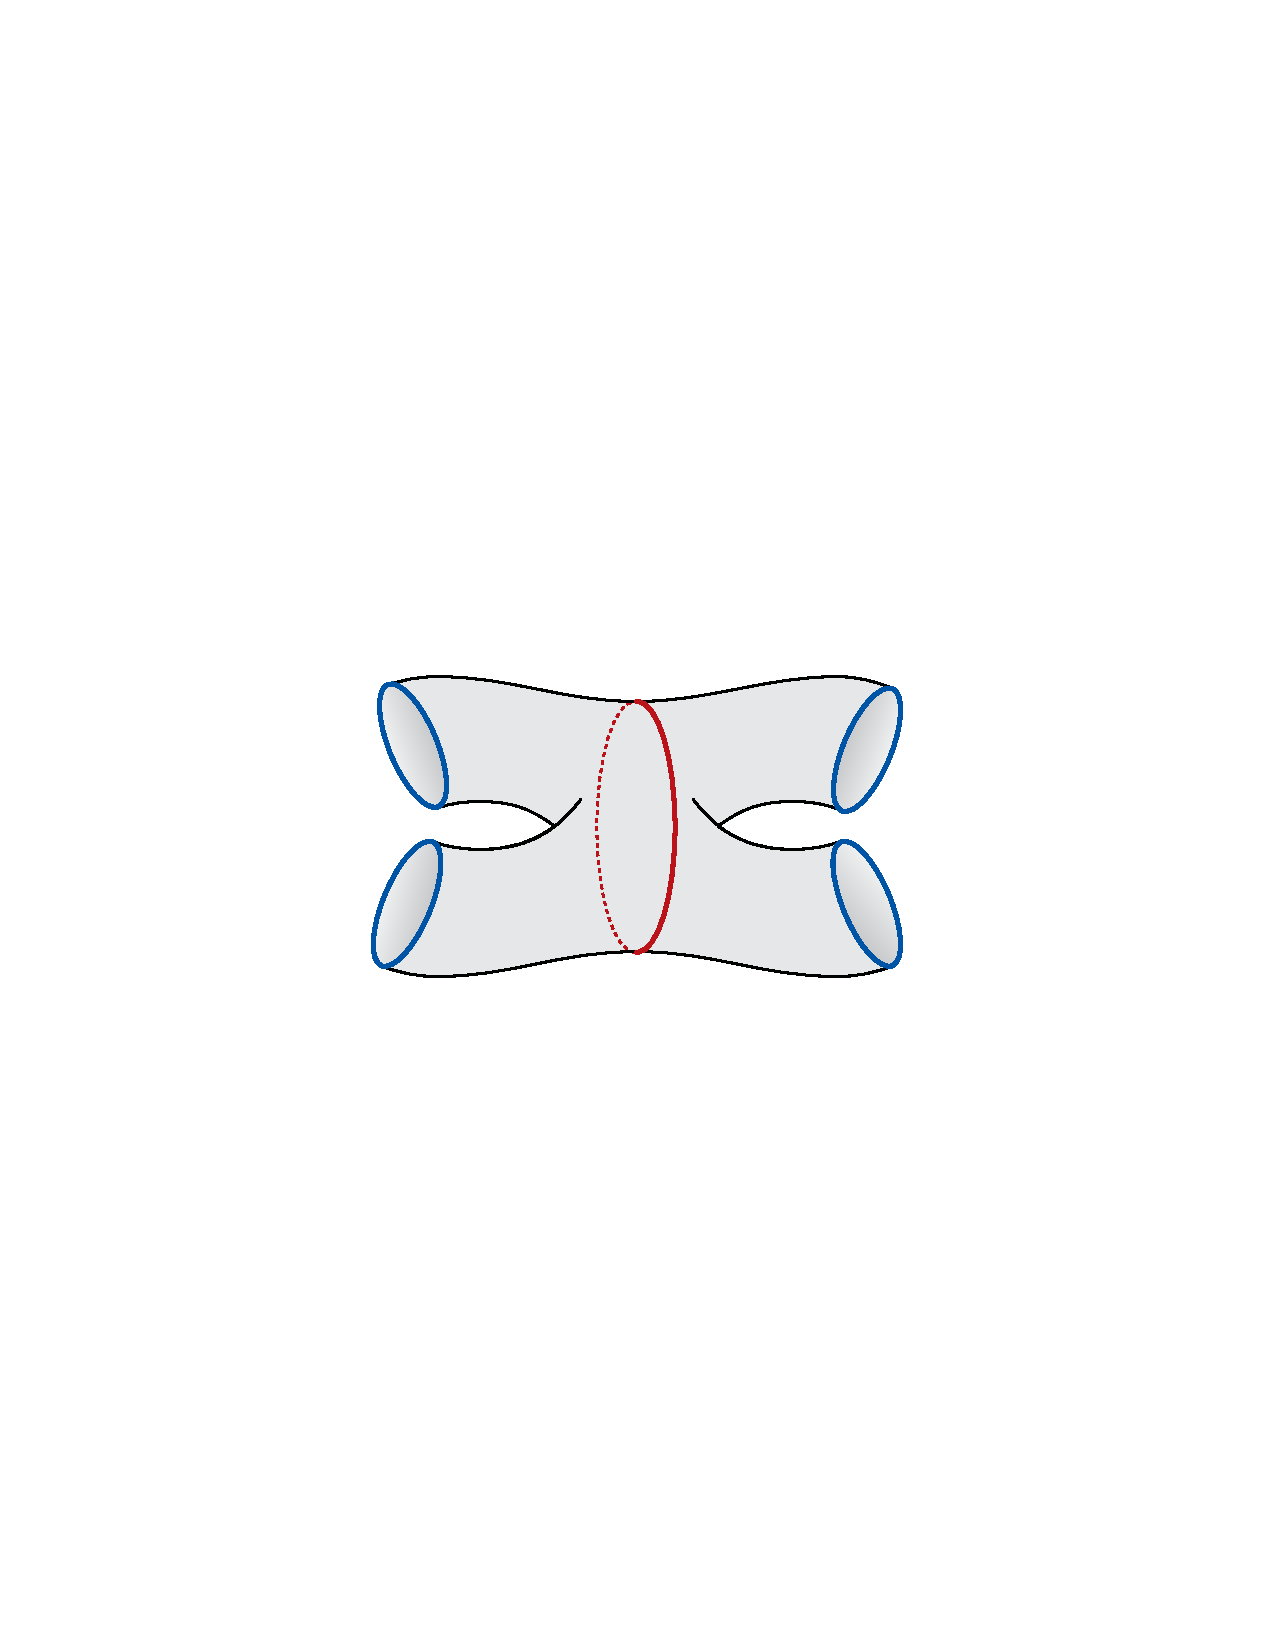
\includegraphics[height=1.25in]{Fig/two-pants}
\caption{The surface obtained after cutting a double torus
along $\alpha_1$ and $\alpha_2$.} \label{F:forbidden-pair}
\end{figure}

Let~$e_1,e_2 \in E(G)$ be two distinct edges in~$\alpha_1$ and~$\alpha_2$
respectively. Let~$e'_1$, $e''_1$, $e'_2$, and~$e''_2$ be their corresponding
edges in~$\Gsnip$. Let~$\eta_{11}$, $\eta_{12}$, $\eta_{21}$, and~$\eta_{22}$ be the
shortest even subgraphs homologous to $\alpha'_1 \oplus \alpha''_1$
in~$\Gsnip \setminus \set{e'_1,e'_2}$,
$\Gsnip \setminus \set{e'_1,e''_2}$,
$\Gsnip \setminus \set{e''_1,e'_2}$,
and~$\Gsnip \setminus \set{e''_1,e''_2}$
respectively if they exist.
We can find these even subgraphs in~$g^{O(g)}n \log \log n$ time
using the modification of Italiano \etal~\cite{insw-iamcmf-11}
to the algorithm of Chambers, Erickson, and Nayyeri~\cite{cen-mcshc-09}.
Let~$\eta'$ be the
shortest subgraph that exists of these four. If no such subgraph exists, then we
report there is no non-empty even subgraph that separates~$\alpha_1$
and~$\alpha_2$ in~$G$.

Suppose without loss of generality that~$\eta' = \eta_{11}$. Both~$e'_1$ and~$e'_2$
lie on boundary cycles of~$\Gsnip$ so they are incident to unique
faces~$f_1$ and~$f_2$ respectively. Face~$f_1$ must lie in the same component
of~$\Sigma_{\subsnip} \setminus \eta'$ as~$\alpha'_1 \oplus \alpha''_1$,
because~$\eta'$ must avoid~$e'_1$.
Likewise,~$f_2$ must lie in the opposite component
of~$\Sigma_{\subsnip} \setminus \eta'$.
Therefore,~$\eta'$ corresponds to an even subgraph~$\eta$ of~$G$ that separates the
surface so that~$f_1$ lies in the same component of~$\Sigma \setminus \eta$
as~$\alpha_1$ and~$f_2$ lies in the same component of~$\Sigma \setminus \eta$
as~$\alpha_2$. The subgraph~$\eta$ must be non-empty.

Since~$\sigma$ is weakly simple in~$G$, it must avoid one of~$e'_1$ or~$e''_1$ and
one of~$e'_2$ or~$e''_2$ in~$\Gsnip$. Consequently,~$\sigma$ is not shorter
than~$\eta$, making~$\eta$ a valid output to our subroutine. We may now proceed to
prove Lemma~\ref{L:split-alg}.

\begin{proof}
We begin by enumerating the $2^{O(g)}$ pairs of distinct nontrivial $\Z_2$-homology classes in $G$.  For each pair of classes, we find the minimum even subgraphs $\eta_1$ and $\eta_2$ in those classes in $g^{O(g)}n \log \log n$ time using the modification of the algorithm of Chambers~\etal~\cite{cen-mcshc-09} by of Italiano \etal~\cite{insw-iamcmf-11}.  Both even subgraphs $\eta_1$ and~$\eta_2$ can be decomposed into edge-disjoint, non-crossing, weakly simple cycles \cite[Lemma 3.2]{cen-mcshc-09}.  Let $\alpha_1$ and~$\alpha_2$ be arbitrary cycles from some cycle decompositions of $\eta_1$ and~$\eta_2$, respectively.  If these cycles cross, then we disregard $\eta_1$ and $\eta_2$ and continue with the next pair of homology classes.  Otherwise, we find the minimum non-empty even subgraph~$\gamma$ that separates $\alpha_1$ and~$\alpha_2$ in $g^{O(g)} n \log \log n$ time using the subroutine above.  After enumerating all pairs of even subgraphs, return the smallest subgraph $\gamma$ found.  All of the subgraphs returned by the subroutine are splitting subgraphs.

Corollary \ref{C:split} implies that at least one pair of even subgraphs $\eta_1$ and $\eta_2$ from the enumeration lie on opposite sides of some smallest splitting subgraph~$\sigma$.  It follows that $\sigma$ also separates the cycles $\alpha_1$ and $\alpha_2$ taken from the cycle decompositions of $\eta_1$ and $\eta_2$ respectively.  As $\alpha_1$ and $\alpha_2$ lie in different components of $\Sigma \setminus \sigma$, they cannot cross.
\end{proof}


\section{Conclusion and Open Problems}

By returning the smallest result from the algorithms described by
Lemmas~\ref{L:minimum-cycle}, \ref{L:contractible-alg}, and~\ref{L:split-alg},
we immediately obtain our main results.

\begin{theorem}
  A minimum-weight separating subgraph of an undirected $n$-vertex
  graph embedded on an orientable surface of genus~$g$ can be computed
  in $g^{O(g)} n \log \log n$ time.
\end{theorem}

\begin{corollary}
  A global minimum- cut in an undirected $n$-vertex graph embedded on
  an orientable surface of genus~$g$ can be computed in 
  $g^{O(g)} n \log \log n$ time.
\end{corollary}

Our algorithm repeatedly applies two recent $O(n\log\log n)$-time algorithms for planar graphs as black boxes: one due to Łącki and Sankowski for global minimum cuts~\cite{ls-mcsc-11} and another due to  Italiano \etal~for minimum $(s,t)$-cuts~\cite{insw-iamcmf-11}.  Indeed, these are the only subroutines in our algorithm that require more than linear time when the genus is fixed.  Thus, improvements to both of these algorithms would immediately improve our algorithm as well.

Although our algorithm works in near-linear time for graphs of constant genus, the complexity dependence on the genus is exponential.  This exponential dependence is unavoidable with our current technique, as our algorithm calls a subroutine that solves an NP-hard problem: finding the minimum-weight subgraph in a given $\Z_2$-homology class \cite{cen-mcshc-09}.  We optimistically conjecture that global minimum cuts in surface graphs can be computed in $O(g^k n \log\log n)$ time for some small constant $k$, using different techniques.

\medskip
\paragraph{Acknowledgment.} The authors would like to thank the anonymous
reviewers for their helpful suggestions on improving this paper.

\bibliographystyle{newabuser}
\bibliography{topology,data-structures,optimization}
\end{document}

